\subsection{Derivative Filters}

\subsubsection{}
Code used to compute the gradient and magnitude and display the quiver thing.
Could unfortunately not figure out how to save the quiver because octave doesn't quite have all the features of matlab.
\inputminted[linenos=true]{octave}{../code/2.4.m}

\subsubsection{}
The magnitude image is displayed in Figure~\ref{fig:2-4-1}.

\begin{figure}[H]
    \centering
    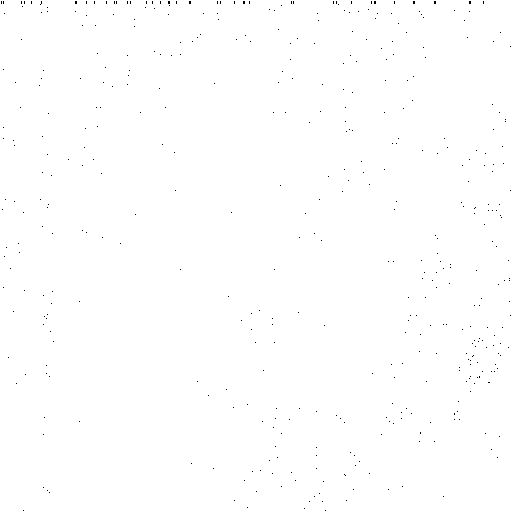
\includegraphics[width=0.5\textwidth]{../code/2_out/2-4_mag.png}

    \caption{The magnitude image of lena.png}
    \label{fig:2-4-1}
\end{figure}

\subsubsection{}
There's no picture here as when I tried to save it all I got was a completely black image.
